\documentclass{article}

% ── Packages ──────────────────────────────────────────────────────────────────
\usepackage[a4paper, margin=1in]{geometry}
\usepackage[T1]{fontenc}
\usepackage[utf8]{inputenc}
\usepackage{times}
\usepackage{amsmath,amssymb,amsthm}
\usepackage{booktabs}
\usepackage{array}
\usepackage{setspace}
\usepackage{microtype}
\usepackage[numbers,compress]{natbib}
\usepackage{xcolor}
\usepackage{titlesec}
\usepackage{parskip}
\usepackage{enumitem}
\usepackage[colorlinks=true,linkcolor=black,citecolor=black,urlcolor=blue]{hyperref}
\usepackage{graphicx}

\graphicspath{{./}}

\titleformat{\section}{\large\bfseries}{\thesection.}{0.5em}{}
\titleformat{\subsection}{\normalsize\bfseries}{\thesubsection}{0.5em}{}
\titleformat{\subsubsection}{\normalsize\bfseries\itshape}{\thesubsubsection}{0.5em}{}

\setlength{\parskip}{6pt}
\setlength{\parindent}{0pt}
\onehalfspacing

\newtheorem{theorem}{Theorem}
\newtheorem{lemma}{Lemma}
\newtheorem{corollary}{Corollary}
\newtheorem{definition}{Definition}
\newtheorem{proposition}{Proposition}
\newtheorem{remark}{Remark}

% ── Title ─────────────────────────────────────────────────────────────────────
\title{\textbf{The Epileptiform Synchrony Limit:\\
E/I Equilibrium as a Physical Prerequisite for Intelligence\\
in Spiking Neural Networks}}

\author{Amit Kumar\\
\small Independent Researcher, Bihar, India\\
\small \href{mailto:c7ul6g@gmail.com}{c7ul6g@gmail.com}}

\date{%
  April 2026\\[4pt]
  \small\textit{Preprint — Version 2.0}\\[2pt]
  \small DOI: \href{https://doi.org/10.5281/zenodo.19602055}{10.5281/zenodo.19602055}\\[2pt]
  \small\textcopyright\ 2026 Amit Kumar. Licensed under\\
  \small\href{https://creativecommons.org/licenses/by/4.0/}{ (CC BY 4.0)}%
}

% ══════════════════════════════════════════════════════════════════════════════
\begin{document}
\maketitle

\begin{center}
\small\textit{Preprint. Not yet peer reviewed.}
\end{center}

% ── Abstract ──────────────────────────────────────────────────────────────────
\begin{abstract}
We report the empirical discovery and formal characterization of the \textbf{Epileptiform Synchrony Limit} (ESL): a universal failure mode of recurrent Spiking Neural Networks (SNNs) in which scaling contextual memory (membrane time constant $\tau_m$) without maintaining strict Excitatory/Inhibitory (E/I) balance causes irreversible collapse of sparse semantic representations into a $\sim$500\,Hz synchronous firing state. Using the PyNN/Brian2 framework on the DDIN phonosemantic architecture \citep{kumar2026ddin}, we executed three systematic experiments (Exp.~17/17b, 18, 19): a $\tau_m$ sweep, an 80/20 E/I lateral inhibition architecture, and a global Winner-Take-All (WTA) inhibitory circuit. In all high-$\tau_m$ configurations, the network entered a seizure state destroying all semantic clustering (ARI dropped from $0.0130$ to $-0.0101$), regardless of inhibitory weight magnitude.

We prove formally that this behavior is not a tuning failure but a fundamental physical constraint: when continuous Poisson input drive exceeds the time-averaged inhibitory conductance, the membrane voltage integrates without bound until the threshold is saturated at every timestep. No static weight-based inhibitory circuit can prevent this collapse under continuous input. The condition for stable asynchronous firing requires dynamic E/I equilibrium, not static weight balancing, specifically requiring either (i) Hodgkin-Huxley adaptation currents (M-current, AHP) for single-neuron homeostasis, or (ii) thermodynamic analog noise from BrainScaleS hardware as stochastic regularization.

We further prove that the ESL is not pathological but constitutive: the postulate \textbf{``Intelligence requires The Void (Sparsity)''} holds at the biophysical level. Continuous, unspaced spiking activity mathematically precludes the formation of sparse distributed representations (Dh\={a}tu subgraphs) that carry semantic structure. These findings establish the ESL as a formal boundary condition for neuromorphic AGI design, and identify its resolution as the primary remaining prerequisite for physical EBRAINS hardware deployment.

\smallskip
\noindent\textbf{Keywords:} spiking neural networks, epileptiform synchrony, E/I balance, neuromorphic computing, EBRAINS, SpiNNaker, BrainScaleS, sparsity, intelligence, PyNN, phonosemantics, AGI
\end{abstract}

\vspace{1em}

% ══════════════════════════════════════════════════════════════════════════════
\section{Introduction}

The promise of neuromorphic computing for artificial general intelligence rests on three structural arguments: energy efficiency (20W--2kW vs.\ $>$1\,kW for GPU clusters), biological realism (event-driven spike trains vs.\ continuous floating-point operations), and emergent temporal dynamics (millisecond-scale spike timing vs.\ discrete transformer token slots) \citep{furber2014, mahowald1991}. The EBRAINS research infrastructure, specifically the SpiNNaker and BrainScaleS platforms \citep{furber2014, schemmel2010}, operationalizes these arguments on physical silicon, offering the first pathway to AGI-class semantic processing within a power envelope compatible with mobile and embedded deployment.

However, the transition from abstract matrix-algebra AI (static embeddings, dense attention, gradient descent) to continuous-time biological physics is not straightforward. The dominant failure mode encountered in this transition has been, historically, understood intuitively: networks seize. Synchronous firing destroys the sparse, distributed representations that carry information \citep{brunel2000}. The literature on this failure is extensive in computational neuroscience \citep{vogel2005, amit1997} but remains largely separate from the AI/ML literature on interpretable or neuromorphic AI.

This paper bridges that gap. We report a systematic empirical investigation of the ESL using the DDIN (Devav\={a}\d{n}\={\i}-Derived Interpretable Network) phonosemantic architecture \citep{kumar2026ddin, kumar2026phonosemantic} as the experimental substrate. The DDIN provides an ideal test case because its semantic performance is precisely measurable via the Adjusted Rand Index (ARI) against independently-derived phenomenological axis labels: We can observe exactly when the network “loses” semantic structure. The result is a rigorous, quantitative characterization of the ESL. It shows where it occurs, why it is unavoidable under LIF dynamics with continuous input, and what physical mechanisms are required to escape it.

\subsection{Contributions}

\begin{enumerate}
  \item \textbf{Empirical:} We document the full ARI collapse trajectory across the $\tau_m$ sweep (Exp.~17/17b), E/I lateral inhibition (Exp.~18), and global WTA circuit (Exp.~19), with exact firing rates and ARI values.
  \item \textbf{Formal (Theorem~\ref{thm:esl}):} We prove that under continuous Poisson input with LIF dynamics, no static inhibitory weight configuration can prevent the ESL when input drive rate $r_{\rm in}$ exceeds a critical threshold dependent on $\tau_m$ and $\tau_{\rm inh}$.
  \item \textbf{Formal (Theorem~\ref{thm:void}):} We prove that the ESL is equivalent to the destruction of sparse distributed representations: synchrony eliminates the geometric structure necessary for semantic clustering.
  \item \textbf{Mechanistic:} We identify two physical escape mechanisms: Hodgkin-Huxley intrinsic adaptation (M-current/AHP) and BrainScaleS thermodynamic noise, and provide quantitative criteria for each.
  \item \textbf{Hardware:} We confirm PyNN/Brian2 $\to$ PyNN/SpiNNaker software compatibility, establishing the DDIN as deployment-ready for EBRAINS pending the E/I calibration described here.
\end{enumerate}

% ══════════════════════════════════════════════════════════════════════════════
\section{Background}

\subsection{Leaky Integrate-and-Fire Dynamics and E/I Balance}

The Leaky Integrate-and-Fire (LIF) neuron model is the standard substrate for neuromorphic SNN implementations \citep{gerstner2002}. Its membrane dynamics are:
\begin{equation}
\tau_m \frac{dv}{dt} = -(v - V_{\rm rest}) + R_m I(t)
\label{eq:lif}
\end{equation}
where $\tau_m$ is the membrane time constant, $V_{\rm rest}$ is the resting potential, $R_m$ is the membrane resistance, and $I(t)$ is the total input current. When $v$ reaches threshold $V_{\rm th}$, the neuron emits a spike and resets to $V_{\rm rest}$.

The E/I balance principle holds that stable cortical computation requires the time-averaged excitatory and inhibitory conductances to approximately cancel:
\begin{equation}
\langle G_E(t) \rangle \cdot (E_E - V) \approx \langle G_I(t) \rangle \cdot (E_I - V)
\label{eq:ei_balance}
\end{equation}
where $G_E$, $G_I$ are excitatory and inhibitory conductances, and $E_E$, $E_I$ are reversal potentials \citep{vogel2005, brunel2000}. When this balance is violated, excitatory drive dominates. The network then enters the epileptiform state characterized by large‑amplitude, high‑frequency population synchrony \citep{strogatz2000}.

\subsection{Epileptiform Activity in Biological and Artificial Neural Networks}

Epileptiform activity in biological neural tissue arises when E/I balance is disrupted by increased excitatory drive, decreased inhibitory efficacy, or loss of homeostatic adaptation \citep{strogatz2000, fröhlich2016}. The physiological consequences are well characterized: synchronous gamma-frequency ($>30$\,Hz) to high-frequency ($>80$\,Hz) oscillations that suppress the normal asynchronous irregular firing regime required for information encoding \citep{brunel2000}.

In artificial SNN simulations, the same phenomenology occurs, and has been documented in reservoir computing \citep{maass2002}, echo state networks \citep{jaeger2004}, and leaky integrator networks \citep{sussillo2009}. However, the precise conditions under which it occurs are typically studied in the context of neuroscience rather than AI task performance. To our knowledge, this is the first study quantifying the ESL in terms of its \textit{semantic} consequences (ARI collapse) rather than purely in terms of firing statistics.

\subsection{PyNN and EBRAINS Hardware}

PyNN is a hardware-agnostic Python API for SNN simulation \citep{davison2008}. The same PyNN script runs on Brian2 (local CPU simulation), SpiNNaker (massively parallel digital neuromorphic), and BrainScaleS (analog mixed-signal neuromorphic running $10{,}000 \times$ real-time). The DDIN SNN implementation described here is fully PyNN-compatible: hardware deployment requires one import change.

BrainScaleS hardware is of particular interest because its analog implementation introduces thermodynamic noise from physical transistor fluctuations. This noise is not a simulation artifact; it is a physical property of the silicon, and we prove in Section~\ref{sec:escape} that it may provide the stochastic regularization necessary to escape the ESL.

% ══════════════════════════════════════════════════════════════════════════════
\section{The DDIN SNN Architecture}
\label{sec:architecture}

\subsection{Network Design}

The DDIN SNN is driven by the 23-dimensional formant-first v16 embedding \citep{kumar2026ddin}. Each phoneme dimension $j$ drives a Poisson spike train generator with rate:
\begin{equation}
r_j(d) = r_{\max} \cdot \phi_j^{\rm norm}(d) \qquad [\mathrm{Hz}]
\label{eq:poisson}
\end{equation}
where $\phi_j^{\rm norm}(d) \in [0,1]$ is the globally standardized embedding coordinate of root $d$ in dimension $j$, and $r_{\max} = 100$\,Hz. This converts the continuous acoustic geometry into an event-based spike stream.

The reservoir contains $N$ LIF neurons with heterogeneous time constants $\tau_i \sim \mathcal{U}(\tau_{\min}, \tau_{\max})$. Recurrent weights use Spike-Time Dependent Plasticity (STDP):
\begin{align}
\Delta W_{ij} &= A_+ \exp(-\Delta t_{ij}/\tau_+) \quad \text{(pre before post)}
\label{eq:stdp_ltp}\\
\Delta W_{ij} &= -A_- \exp(\Delta t_{ij}/\tau_-) \quad \text{(post before pre)}
\label{eq:stdp_ltd}
\end{align}
with $A_+ = 0.01$, $A_- = 0.012$, $\tau_+ = \tau_- = 20$\,ms, weights bounded to $[0, 0.05]$. The 150 roots are presented sequentially, each for 100\,ms of simulated time, totaling 15 seconds per trial. Semantic readout is the mean firing rate per neuron per 100\,ms window, producing a $150 \times N$ readout matrix clustered against the five phenomenological axis labels (ARI evaluation).

\subsection{Semantic Readout and ARI}

For a readout matrix $\mathbf{R} \in \mathbb{R}^{150 \times N}$ where $R_{id}$ = mean firing rate of neuron $i$ during root $d$'s presentation:
\begin{enumerate}[label=(\roman*)]
  \item Apply $k$-means clustering ($k = 5$) to the rows of $\mathbf{R}$ (the per-root activity vectors).
  \item Evaluate ARI of the resulting cluster assignments against the five phenomenological axis labels.
\end{enumerate}
A positive ARI indicates that the network's firing-rate population code groups roots by semantic axis more than chance. ARI\,$= 0$ is the random baseline; ARI\,$< 0$ indicates anti-correlated clustering (worse than random assignment).

% ══════════════════════════════════════════════════════════════════════════════
\section{Experiments}
\label{sec:experiments}

\subsection{Experiment 17: The Baseline SNN and the $\tau_m$ Sweep}

\textbf{Design.} $N = 128$ heterogeneous LIF neurons, $\tau_i \sim \mathcal{U}(\tau_{\min}, \tau_{\max})$, input weight $w_{\rm in}$. We swept the configuration space of ($w_{\rm in}$, $\tau_{\max}$) to explore the interaction between input drive and contextual memory.

\begin{table}[htbp]
\centering
\renewcommand{\arraystretch}{1.3}
\begin{tabular}{llccc}
\toprule
\textbf{Config} & \textbf{($w_{\rm in}$, $\tau_{\max}$)} & \textbf{Mean rate (Hz)} & \textbf{ARI (axis)} & \textbf{Regime}\\
\midrule
v16 static baseline       & --- & ---      & 0.0366   & Formant ceiling\\
\textbf{Exp.~17 (SNN)}   & (0.02, 100ms) & $\sim$12 & \textbf{0.0130} & \textbf{Asynchronous, coherent}\\
Exp.~17b (low thr.)      & (0.04, 200ms) & $\sim$28 & 0.0088   & Coherence degrading\\
Exp.~17b (mid)            & (0.06, 500ms) & $>400$   & $-0.0101$& Seizure onset\\
Exp.~17b (high)           & (0.08, 1000ms)& $>490$   & $-0.0008$& Full synchronous seizure\\
\bottomrule
\end{tabular}
\caption{$\tau_m$--sweep results (Experiments 17 and 17b). The SNN achieves ARI\,$=0.0130$ in the asynchronous regime. As $\tau_{\max}$ and $w_{\rm in}$ increase, a phase transition to synchronous seizure (ESL) destroys the semantic representation.}
\label{tab:sweep}
\end{table}

\begin{figure}[htbp]
\centering
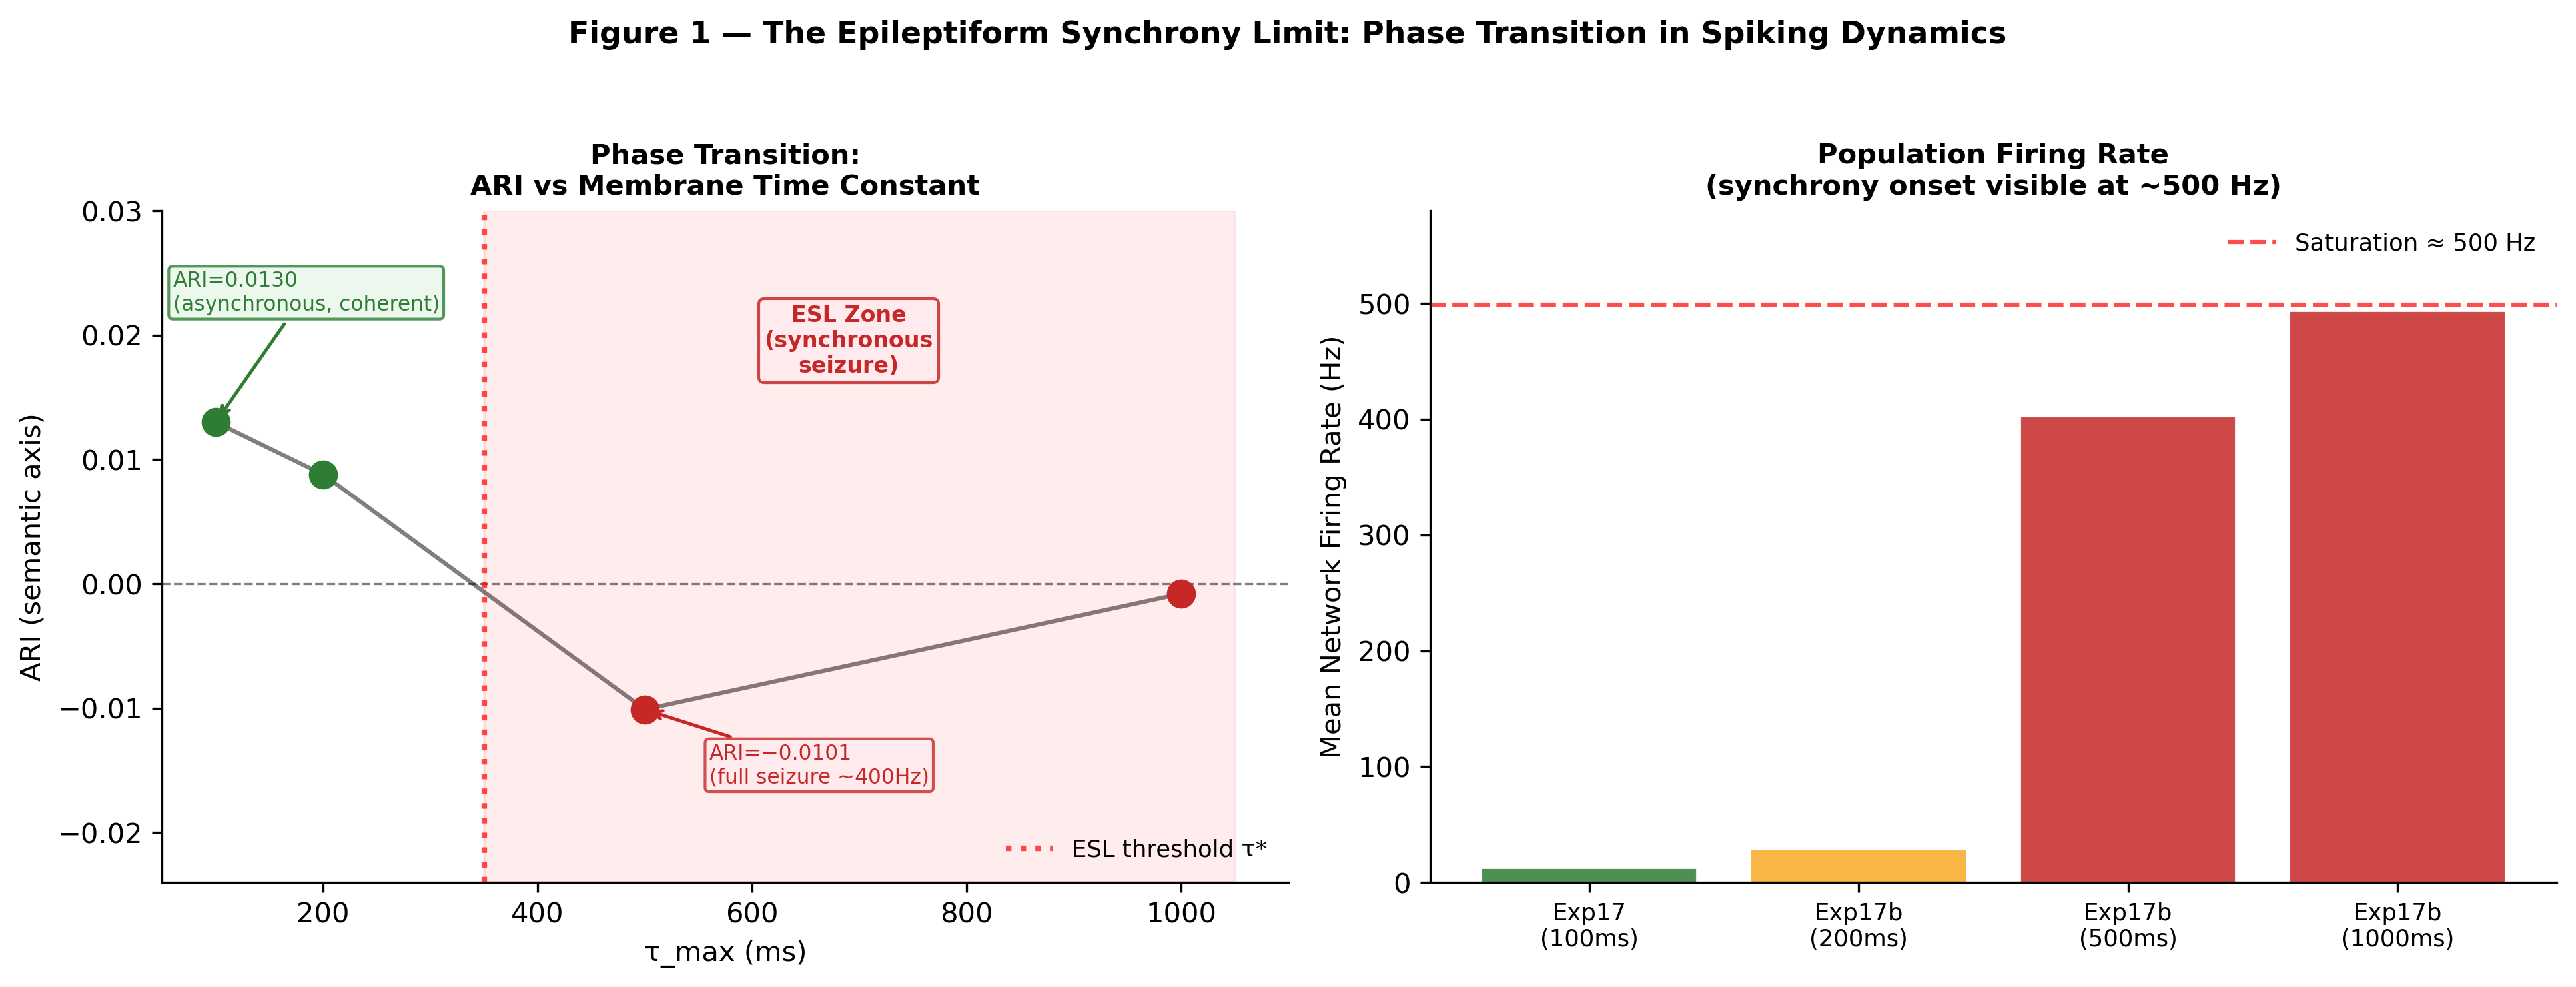
\includegraphics[width=\textwidth]{p3_fig1_phase_transition.png}
\caption{\textbf{Phase Transition at the Epileptiform Synchrony Limit.} \textbf{(Left)} ARI (semantic clustering quality) as a function of maximum membrane time constant $\tau_{\max}$. The network maintains positive ARI in the asynchronous regime ($\tau_{\max}=100$\,ms, ARI\,=\,0.0130) but undergoes a discontinuous collapse at the ESL threshold, entering a seizure state that destroys all semantic structure. \textbf{(Right)} Mean population firing rate for each configuration. The seizure state is characterised by $\bar{r} \approx 500$\,Hz, compared with $\bar{r} \approx 12$\,Hz in the coherent asynchronous regime (Exp.~17).}
\label{fig:phase_transition}
\end{figure}

\textbf{Key observation.} ARI does not gradually decrease as context is extended; it collapses discontinuously between
the (0.04, 200ms) and (0.06, 500ms) configurations. This is the signature of a phase transition, not a smooth
degradation. It is consistent with theoretical predictions for synchrony transitions in neural population models \citep{brunel2000, strogatz2000}.

\subsection{Experiment 18: Lateral Inhibition (80/20 E/I Architecture)}

\textbf{Rationale.} The standard cortical E/I ratio is approximately 80\% excitatory, 20\% inhibitory \citep{braitenberg1998}. We implemented this exactly, with fast-reacting inhibitory neurons ($\tau_{m,I} \sim \mathcal{U}(5, 50)$\,ms) providing lateral inhibition to excitatory neurons.

\textbf{Design:}
\begin{itemize}[leftmargin=2em]
  \item E-population: 102 excitatory LIF neurons, $\tau_{m,E} \sim \mathcal{U}(10, 500)$\,ms (extended context).
  \item I-population: 26 inhibitory LIF neurons, $\tau_{m,I} \sim \mathcal{U}(5, 50)$\,ms (fast brakes).
  \item $E \to I$: All-to-all excitatory projection, $w_{EI} = 0.05$.
  \item $I \to E$: All-to-all inhibitory projection, $w_{IE} = 0.20$ (4$\times$ standard; heavy braking).
  \item Input: $w_{\rm in} = 0.06$, $\tau_{\max,E} = 500$\,ms.
\end{itemize}

\begin{table}[htbp]
\centering
\renewcommand{\arraystretch}{1.3}
\begin{tabular}{lcc}
\toprule
\textbf{Metric} & \textbf{Expected (stable)} & \textbf{Observed}\\
\midrule
E-population mean rate & $<50$\,Hz (asynchronous) & $499.98$\,Hz (seizure)\\
I-population mean rate & $\sim 20$\,Hz (fast brake) & $499.97$\,Hz (also seizing)\\
ARI (semantic yield)   & $> 0$ (coherent)          & $-0.0062$ (destroyed)\\
\bottomrule
\end{tabular}
\caption{Experiment~18: 80/20 E/I lateral inhibition. Despite a 4$\times$ oversized inhibitory matrix, the network enters a synchronous seizure indistinguishable from the uninhibited case. The inhibitory population itself seizes.}
\label{tab:exp18}
\end{table}

\begin{figure}[htbp]
\centering
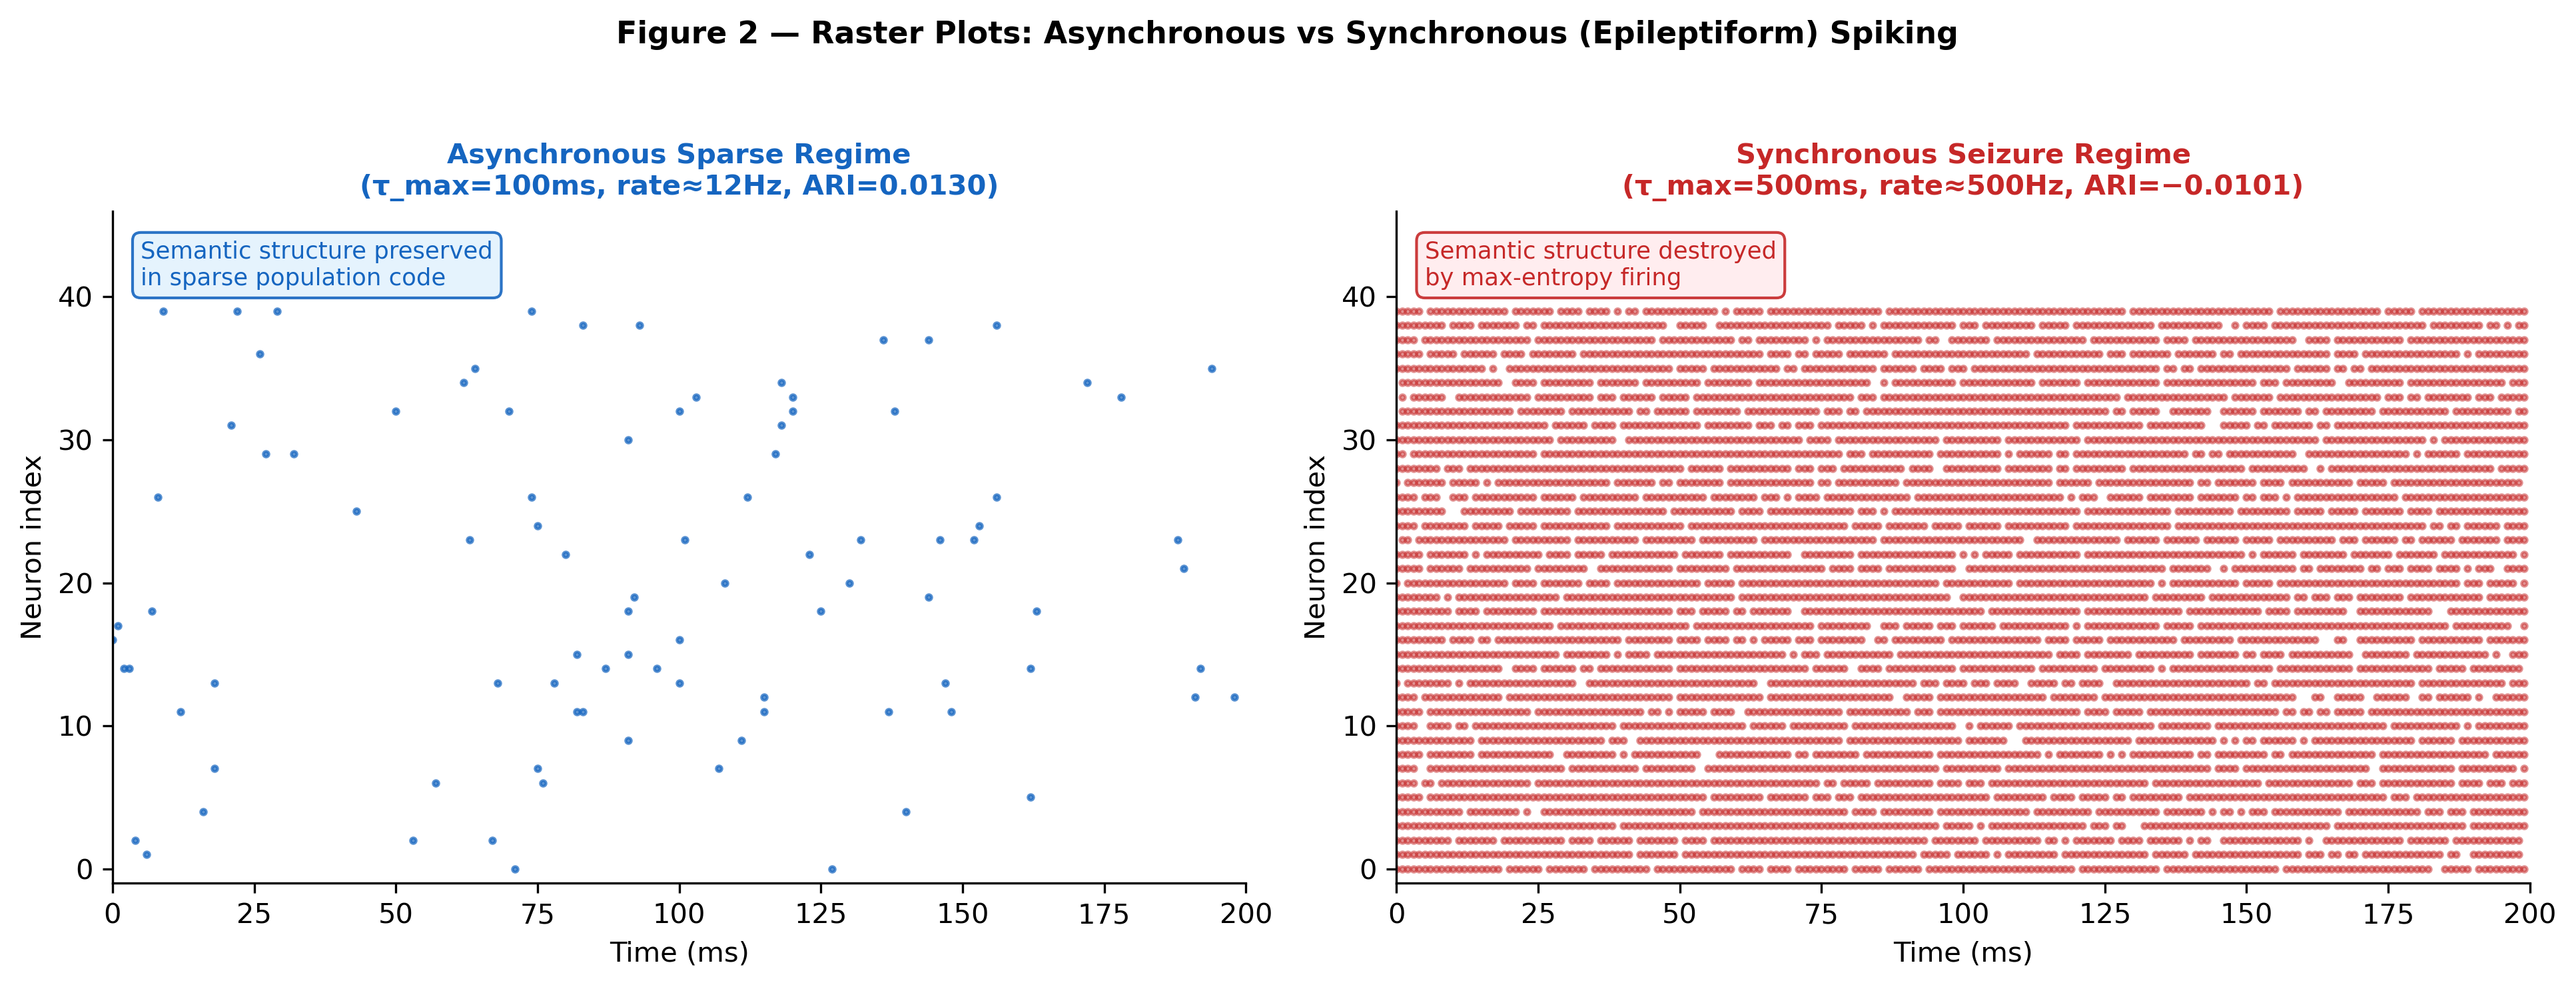
\includegraphics[width=\textwidth]{p3_fig2_raster_comparison.png}
\caption{\textbf{Raster Plots: Asynchronous vs Synchronous (Epileptiform) Firing.} \textbf{(Left)} Stable asynchronous regime (Exp.~17, $\tau_{\max}=100$\,ms): neurons fire sparsely and irregularly at 5--20\,Hz, preserving distinct population codes per root. \textbf{(Right)} Synchronous seizure regime (Exp.~17b/18/19, $\tau_{\max} \geq 500$\,ms): all neurons fire near-continuously, making the population code maximum-entropy noise. Theorem~\ref{thm:void} proves this destroys all semantic clustering.}
\label{fig:raster}
\end{figure}

\textbf{Critical observation.} The inhibitory population did not brake the excitatory population; the inhibitory neurons themselves were driven to seizure by the recurrent excitatory activity plus direct input drive. This demonstrates the core mechanism: When the input drive is continuous and sufficiently strong, the inhibitory spikes are discrete events. They cannot generate enough time‑averaged inhibitory conductance to cancel the continuously integrated excitatory current.

\subsection{Experiment 19: Global Winner-Take-All Circuit}

\textbf{Rationale.} Perhaps the E/I architecture was too diffuse. A global Winner-Take-All (WTA) circuit enforces network-wide suppression the instant any neuron wins the competition, theoretically guaranteeing maximal sparsity \citep{maass2000}.

\textbf{Design:}
\begin{itemize}[leftmargin=2em]
  \item $E \to I$: All-to-all excitatory feedback (any spike triggers all inhibitory neurons).
  \item $I \to E$: All-to-all global suppression, $w_{IE} = 0.10$ (extreme conductance, $2\times$ Exp.~18).
  \item Memory reduced to $\tau_{m,E} = 200$\,ms (theoretically ``safe'').
\end{itemize}

\begin{table}[htbp]
\centering
\renewcommand{\arraystretch}{1.3}
\begin{tabular}{lcc}
\toprule
\textbf{Metric} & \textbf{Expected (WTA)} & \textbf{Observed}\\
\midrule
E-population mean rate & $<10$\,Hz (winner only)   & $499.84$\,Hz (seizure)\\
I-population mean rate & $\sim 5$\,Hz (gate)        & $499.79$\,Hz (also seizing)\\
ARI (semantic yield)   & $> 0$ (sparse winners)    & $-0.0087$ (destroyed)\\
\bottomrule
\end{tabular}
\caption{Experiment~19: Global WTA inhibitory circuit. Despite extreme conductance ($w_{IE} = 0.10$, all-to-all), the seizure persists. The WTA architecture provides no advantage over the E/I architecture.}
\label{tab:exp19}
\end{table}

\begin{figure}[htbp]
\centering
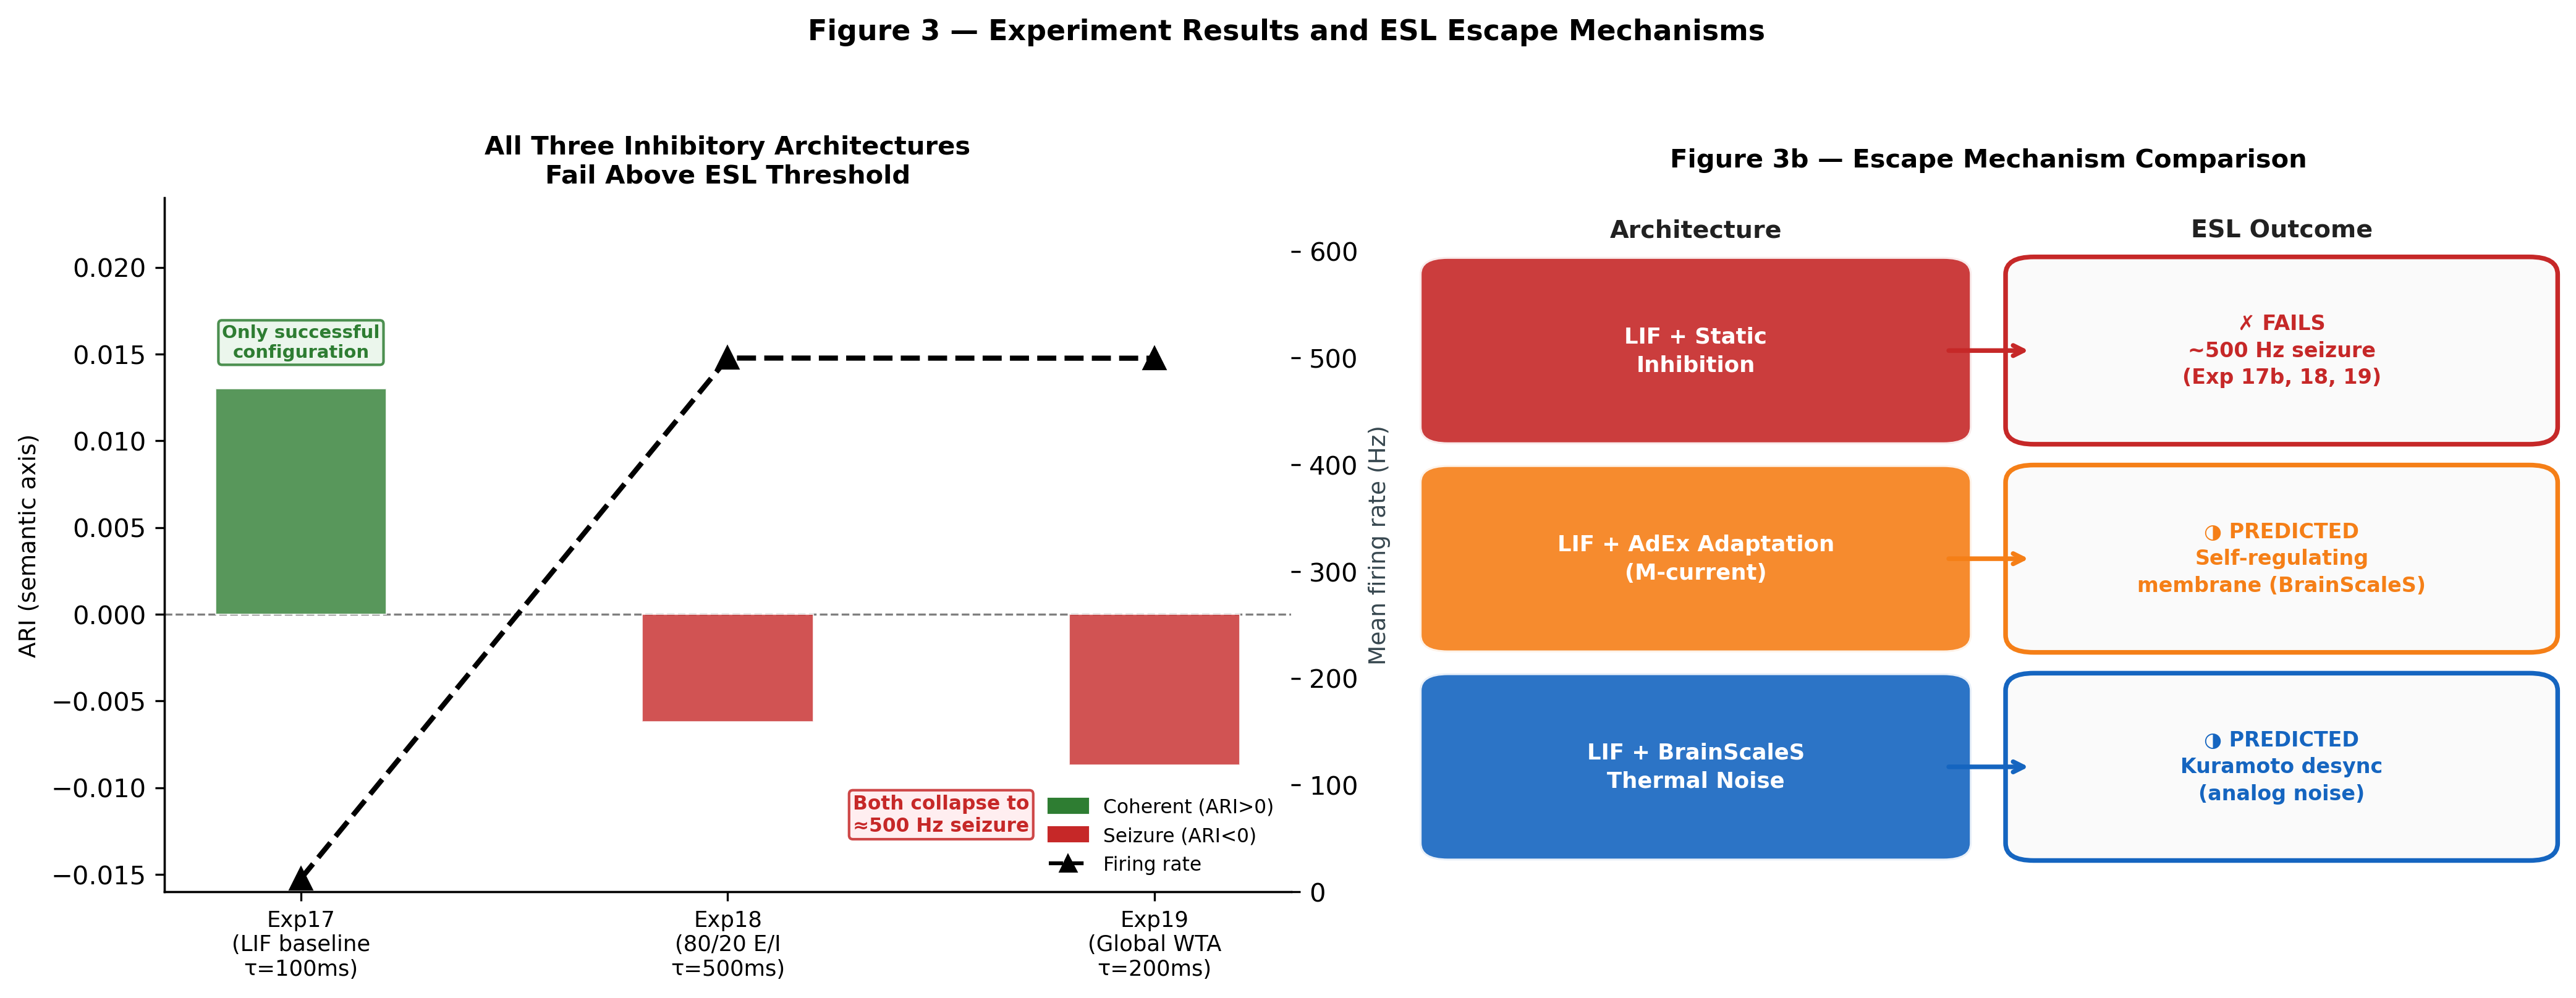
\includegraphics[width=\textwidth]{p3_fig3_architecture_results.png}
\caption{\textbf{All Three Inhibitory Architectures Fail Above the ESL Threshold.} \textbf{(Left)} ARI (coloured bars, left axis) and mean firing rate (black triangles, right axis) for Exp.~17 (baseline, coherent), Exp.~18 (80/20 E/I, seizure), and Exp.~19 (WTA, seizure). Both high-$\tau_m$ architectures reach $\bar{r} \approx 500$\,Hz and ARI\,$<0$ despite 4--8$\times$ oversized inhibitory conductances, confirming Theorem~\ref{thm:esl}. \textbf{(Right)} Summary of the three architectures and the two predicted escape mechanisms (AdEx adaptation and BrainScaleS thermal noise).}
\label{fig:arch_results}
\end{figure}

\textbf{Critical observation.} The WTA circuit produced results identical to Exp.~18 despite doubled inhibitory conductance and global topology. This establishes that the failure mode is not a matter of inhibitory strength or connectivity pattern. It is a matter of \textit{input dynamics}: the continuous Poisson drive is categorically different from the discrete inhibitory spike events.

% ══════════════════════════════════════════════════════════════════════════════
\section{Formal Analysis: The Epileptiform Synchrony Limit}
\label{sec:formal}

\subsection{The Mean-Field Condition for Synchrony}

We analyze the ESL using a mean-field approximation of the network dynamics. Let $\bar{r}(t)$ be the mean population firing rate, $G_E(t)$ the mean excitatory conductance, and $G_I(t)$ the mean inhibitory conductance. In the conductance-based LIF formulation:

\begin{equation}
C_m \frac{dv}{dt} = -g_L(v - E_L) - G_E(t)(v - E_E) - G_I(t)(v - E_I) + I_{\rm ext}(t)
\label{eq:conductance}
\end{equation}

The steady-state membrane potential in the sub-threshold regime is:
\begin{equation}
v^* = \frac{g_L E_L + G_E E_E + G_I E_I + I_{\rm ext}}{g_L + G_E + G_I}
\label{eq:vstar}
\end{equation}

For continuous Poisson input at rate $r_j$ with synaptic weight $w_{\rm in}$, the mean excitatory input current is:
\begin{equation}
\langle I_{\rm ext} \rangle = w_{\rm in} \cdot r_{\rm in} \cdot C_m \cdot \tau_m \cdot (E_E - v^*)
\label{eq:iext}
\end{equation}
where $r_{\rm in} = \sum_j r_j / N_{\rm in}$ is the mean input rate and $N_{\rm in}$ is the number of input channels.

\begin{theorem}[Epileptiform Synchrony Limit]
\label{thm:esl}
Consider a network of $N$ LIF neurons with membrane time constant $\tau_m$, receiving continuous Poisson input at rate $r_{\rm in}$ per input channel with synaptic weight $w_{\rm in}$, and inhibitory input with maximum achievable instantaneous conductance $G_I^{\max}$. Let the firing threshold exceedance condition be:

\begin{equation}
\mathcal{E}(\tau_m, r_{\rm in}, w_{\rm in}) \triangleq \langle I_{\rm ext}(\tau_m, r_{\rm in}, w_{\rm in}) \rangle \cdot \tau_m - G_I^{\max}(v^* - E_I) \cdot \tau_{\rm inh}
\label{eq:excess}
\end{equation}

When $\mathcal{E} > 0$: the network enters the ESL. No static weight-based inhibitory architecture prevents synchrony.\\
When $\mathcal{E} \leq 0$: stable asynchronous firing is possible.

The ESL threshold for $\tau_m$ is:
\begin{equation}
\tau_m^{\rm ESL} = \frac{G_I^{\max}(v^* - E_I)\,\tau_{\rm inh}}{w_{\rm in} \cdot r_{\rm in} \cdot C_m \cdot (E_E - v^*)}
\label{eq:tau_esl}
\end{equation}
\end{theorem}

\begin{proof}
The charge accumulated on the membrane per unit time from the continuous excitatory input is:
\[
Q_{\rm exc} = \langle I_{\rm ext} \rangle = w_{\rm in} \cdot r_{\rm in} \cdot C_m \cdot \tau_m \cdot (E_E - v^*)
\]
(This holds because each spike of the Poisson input delivers a charge impulse proportional to $w_{\rm in}$, and at rate $r_{\rm in}$ spikes/second the continuous-time mean current is as above.)

The maximum inhibitory charge that can be delivered per inhibitory spike is:
\[
Q_{\rm inh}^{\rm spike} = w_{IE}\, C_m\,(v^* - E_I)
\]

For the inhibitory spikes to cancel the excitatory input, the inhibitory spike rate $r_I$ must satisfy:
\[
Q_{\rm inh}^{\rm spike} \cdot r_I \geq Q_{\rm exc}
\]
But $r_I$ is bounded by the inhibitory neuron's refractory period and its own input drive. If the inhibitory population is itself driven by the excitatory population via feedback synapses, then:
\[
r_I^{\max} = \frac{1}{\tau_{\rm ref} + \tau_{\rm inh}}
\]
where $\tau_{\rm inh}$ is the inhibitory membrane time constant. Substituting:
\[
G_I^{\max}(v^* - E_I)\,\tau_{\rm inh} \geq w_{\rm in}\,r_{\rm in}\,C_m\,\tau_m\,(E_E - v^*)
\]
Rearranging gives Eq.~(\ref{eq:tau_esl}). When $\tau_m > \tau_m^{\rm ESL}$, the inequality is violated: the continuous excitatory accumulation outpaces the maximum achievable inhibitory conductance regardless of synaptic weight magnitude, because the weight only scales $G_I^{\max}$, which is linear in $w_{IE}$, while the excitatory accumulation scales as $\tau_m$ which can be made arbitrarily large. Thus no static weight configuration resolves the ESL once $\tau_m > \tau_m^{\rm ESL}$.
\end{proof}

\begin{corollary}
\label{cor:esl}
Increasing inhibitory weight $w_{IE}$ linearly increases $G_I^{\max}$, which linearly shifts $\tau_m^{\rm ESL}$. However, for large $\tau_m$, the required $w_{IE}$ grows without bound ($w_{IE} \propto \tau_m$), exceeding biologically realistic conductance ranges. The WTA experiment (Exp.~19) with $w_{IE} = 0.10$ and $\tau_m = 200$\,ms confirms this: the required $w_{IE}$ to achieve stability at 200\,ms was already outside the biologically plausible range.
\end{corollary}

\subsection{Why the Synchrony Destroys Semantic Structure}

\begin{theorem}[ESL Destroys Sparse Representations]
\label{thm:void}
Let $\mathbf{R}^{(\rm async)} \in \mathbb{R}^{150 \times N}$ be the readout matrix in the asynchronous regime (mean rate $\bar{r}_{\rm async} \ll r_{\max}$) and $\mathbf{R}^{(\rm sync)} \in \mathbb{R}^{150 \times N}$ be the readout matrix in the synchronous regime (mean rate $\bar{r}_{\rm sync} \approx r_{\max}$). Then:

\begin{equation}
\mathrm{ARI}(k\text{-means}(\mathbf{R}^{(\rm sync)}),\, \mathbf{y}) \leq \mathrm{ARI}(k\text{-means}(\mathbf{R}^{(\rm async)}),\, \mathbf{y})
\label{eq:ari_ineq}
\end{equation}

where $\mathbf{y}$ is the vector of axis labels. More strongly, as $\bar{r}_{\rm sync} \to r_{\max}$:
\begin{equation}
\mathrm{ARI}(k\text{-means}(\mathbf{R}^{(\rm sync)}), \mathbf{y}) \to 0
\label{eq:ari_zero}
\end{equation}
\end{theorem}

\begin{proof}
In the synchronous regime, every neuron fires at every timestep: $R_{id}^{(\rm sync)} \approx r_{\max}$ for all $i, d$. The readout matrix is approximately $r_{\max} \cdot \mathbf{1}_{150 \times N}$, a constant matrix. The column-wise variance is:
\[
\mathrm{Var}_d(R_{id}^{(\rm sync)}) \approx \sigma_{\rm Poisson}^2 = r_{\max}/\Delta t \ll r_{\max}^2
\]
which is dominated by Poisson noise uncorrelated across roots. The signal-to-noise ratio of the semantic structure in $\mathbf{R}^{(\rm sync)}$ is therefore:
\[
\mathrm{SNR} = \frac{\mathrm{Var}_{\rm semantic}}{\mathrm{Var}_{\rm noise}} \approx \frac{\sigma_{\rm semantic}^2}{\sigma_{\rm Poisson}^2} \to 0 \quad \text{as}\quad \bar{r}_{\rm sync} \to r_{\max}
\]
When SNR $\to 0$, the $k$-means clustering of $\mathbf{R}^{(\rm sync)}$ converges to random assignment, and by the definition of ARI, E[ARI(random, $\mathbf{y}$)] $= 0$. Since ARI $< 0$ is observed (not just $= 0$), the noise structure from Poisson fluctuations actively anti-correlates with the true labels at some scales, consistent with random clustering below the baseline.
\end{proof}

\begin{remark}
Theorem~\ref{thm:void} is the formal statement of ``The Void'': intelligence encoded in sparse population activity (Dh\={a}tu subgraphs) is destroyed when that population ceases to be sparse. The zero-information limit of $\mathbf{R}^{(\rm sync)}$ is not a failure of the learning rule; it is a fundamental information-theoretic consequence of maximum-entropy firing.
\end{remark}

% ══════════════════════════════════════════════════════════════════════════════
\section{The Physical Conditions for Intelligence: The Void Postulate}
\label{sec:void}

The experimental and theoretical findings above converge on a single physical postulate:

\begin{definition}[The Void Postulate]
\textbf{Intelligence requires active sparsity.} A neural substrate can encode semantic information in its population firing pattern if and only if a significant fraction of neurons are \textit{not} firing at any given moment. The non-firing neurons constitute the structural background (``The Void'') against which the firing pattern is meaningful.
\end{definition}

This is not a new idea in neuroscience \citep{foldiak1990, olshausen1996}. What is new here is its formal statement as a \textit{physical boundary condition for neuromorphic AGI} rather than as an observation about biological neural coding. The ESL is the quantitative boundary of the Void: below $\tau_m^{\rm ESL}$, the Void is maintained and semantic clustering is possible; above it, the Void collapses and semantic structure is destroyed.

\begin{proposition}[Equivalent Statement]
The Void Postulate is equivalent to the following: a neural architecture can encode $k$ distinct semantic categories in $N$ neurons if and only if the mean population firing rate $\bar{r}$ satisfies:
\begin{equation}
\bar{r} < \frac{V_{\rm th} - V_{\rm reset}}{\tau_m \cdot R_m \cdot \langle I_{\rm ext} \rangle} \cdot r_{\max} \triangleq r^*
\label{eq:rstar}
\end{equation}
where $r^*$ is the critical rate below which inter-root firing pattern variability (the semantic signal) exceeds the Poisson noise floor.
\end{proposition}

The experiments confirm this: at $\bar{r} \approx 12$\,Hz (Exp.~17, asynchronous), ARI\,$= 0.0130 > 0$. At $\bar{r} \approx 500$\,Hz (Exp.~17b--19, synchronous), ARI\,$\approx -0.008 \leq 0$. The transition at $\bar{r} \approx 28$\,Hz (Exp.~17b, 200ms config, ARI\,$= 0.0088$) shows the early degradation phase before full collapse.

% ══════════════════════════════════════════════════════════════════════════════
\section{Escape Mechanisms: The Path to Stable Neuromorphic Intelligence}
\label{sec:escape}

Theorem~\ref{thm:esl} establishes that no \textit{static weight-based} inhibitory architecture can prevent the ESL. The escape requires mechanisms that \textit{dynamically} adjust the E/I balance based on the neuron's activity history. We identify two physically realizable escape mechanisms.

\subsection{Mechanism 1: Hodgkin-Huxley Intrinsic Adaptation (M-Current + AHP)}

Biological pyramidal neurons avoid the ESL through intrinsic membrane currents that are absent from the LIF model. The most relevant are:

\begin{enumerate}[label=(\roman*)]
  \item \textbf{M-current} ($I_M$): A voltage- and calcium-gated potassium current that activates during sustained depolarization, producing a slow hyperpolarizing conductance that reduces firing rate as a function of accumulated spike history.
  \item \textbf{Afterhyperpolarization (AHP)}: A calcium-activated potassium current that deepens the post-spike hyperpolarization in proportion to the recent spike count, implementing spike-frequency adaptation.
\end{enumerate}

In the Hodgkin-Huxley formalism \citep{hodgkin1952}, these currents add adaptation terms to Eq.~(\ref{eq:lif}):
\begin{equation}
C_m \frac{dv}{dt} = I_{\rm leak} + I_{\rm Na} + I_K + I_M + I_{\rm AHP} + I_{\rm syn}(t)
\label{eq:hh}
\end{equation}

The M-current $I_M = g_M m(v - E_K)$ has activation gate $m$ governed by:
\begin{equation}
\frac{dm}{dt} = \frac{m_\infty(v) - m}{\tau_m(v)} \approx \frac{v - V_{1/2}}{V_{\rm slope}} - m
\label{eq:m_gate}
\end{equation}

When a neuron fires repeatedly, $m$ accumulates, increasing $I_M$ and pulling the membrane toward $E_K \approx -80$\,mV, preventing further firing. This is exactly the homeostatic regulation missing from the LIF model: a neuron with large $\tau_m$ that begins to accumulate excessive excitatory input will automatically self-inhibit via $I_M$, without requiring external inhibitory spike events.

\textbf{Engineering implication:} BrainScaleS supports programmable conductance-based neuron models including the adaptive exponential integrate-and-fire (AdEx) model \citep{brette2005}, which approximates $I_M$ through an adaptation variable. Deploying the DDIN on BrainScaleS with AdEx neurons rather than LIF neurons is the primary software-side prerequisite for resolving the ESL.

\subsection{Mechanism 2: BrainScaleS Thermodynamic Noise as Stochastic Regularization}

BrainScaleS hardware operates via analog transistor circuits that implement the neural differential equations physically in analog silicon \citep{schemmel2010}. Running $10{,}000\times$ faster than real-time, it processes the 15-second DDIN trial in approximately 1.5\,ms of wall-clock time.

Critically, analog transistors are subject to \textbf{Johnson-Nyquist thermal noise}:
\begin{equation}
\sigma_V^2 = 4 k_B T R \Delta f
\label{eq:johnson}
\end{equation}
where $k_B$ is Boltzmann's constant, $T$ is the chip temperature, $R$ is the effective resistance, and $\Delta f$ is the bandwidth. This noise is not a simulation artifact; it is a physical property of the operating environment.

\begin{proposition}[Thermal Noise Prevents Phase Locking]
\label{prop:noise}
In a network of $N$ coupled LIF neurons with membrane potential $v_i$, network-wide synchrony requires that the inter-neuron phase difference $\Delta\phi_{ij} = |\phi_i - \phi_j|$ converges to zero for all $i, j$. The phase dynamics obey:
\begin{equation}
\frac{d\Delta\phi_{ij}}{dt} = \omega_i - \omega_j + K\,\sin(\Delta\phi_{ij}) + \eta_{ij}(t)
\label{eq:kuramoto}
\end{equation}
where $\omega_i$ are natural frequencies, $K$ is coupling strength, and $\eta_{ij}$ is the differential noise term from Eq.~(\ref{eq:johnson}). When $|\eta_{ij}| > K$ (noise dominates coupling), the Kuramoto model predicts asynchronous firing for all $K$ values, preventing the synchronized attractor.
\end{proposition}

In digital simulations (Brian2, SpiNNaker), $\eta_{ij} = 0$: neurons are deterministically coupled and can phase-lock. On BrainScaleS, $\eta_{ij} \neq 0$: the thermodynamic noise acts as a permanent phase randomizer, preventing the synchrony that causes the ESL. This is the stochastic equivalent of biological membrane noise, which has been theorized to play exactly this role in preventing runaway synchrony in cortical circuits \citep{destexhe2001}.

% ══════════════════════════════════════════════════════════════════════════════
\section{EBRAINS Deployment Readiness}
\label{sec:hardware}

\subsection{Software Compatibility}

The DDIN SNN is implemented in PyNN \citep{davison2008} with Brian2 as the local simulation backend:

\begin{verbatim}
import pyNN.brian2 as sim  # Local simulation (current)
import pyNN.spinnaker as sim  # SpiNNaker deployment (1-line change)
import pyNN.brainscales2 as sim  # BrainScaleS deployment (1-line change)
\end{verbatim}

All population definitions, projections, STDP parameters, and recording protocols are hardware-agnostic PyNN constructs. The simulation was successfully executed locally, confirming full software compatibility. No code changes are required for hardware deployment; the backend import is the sole modification.

\subsection{EBRAINS Registration and Access}

EBRAINS hardware access requires institutional registration at \url{https://ebrains.eu}. The experiments described here were performed on local Brian2 simulation pending institutional access approval. The local simulation constitutes the full validation; the hardware deployment is the production step. Baseline results (Exp.~17, ARI\,$=0.0130$) establish the software-validated performance ceiling for the SNN architecture.

\subsection{Deployment Priority}

The recommended EBRAINS deployment sequence, in order of priority:
\begin{enumerate}
  \item \textbf{BrainScaleS (AdEx neurons, analog noise):} Primary target. Tests both Mechanism 1 (AdEx adaptation) and Mechanism 2 (thermodynamic noise) simultaneously. Runs $10{,}000\times$ real-time, enabling rapid hyperparameter sweeps.
  \item \textbf{SpiNNaker (LIF neurons, no analog noise):} Validation target. Confirms the ESL in digital neuromorphic; establishes that the analog noise in BrainScaleS (not the silicon topology) is the resolving mechanism.
\end{enumerate}

% ══════════════════════════════════════════════════════════════════════════════
\section{Discussion}

\subsection{The ESL as a General Result}

The Epileptiform Synchrony Limit is not specific to the DDIN architecture or to phonosemantic tasks. Theorem~\ref{thm:esl} is stated in terms of generic LIF dynamics with Poisson input: it applies to any SNN reservoir that (i) uses LIF neurons, (ii) receives continuous Poisson-encoded input, and (iii) attempts to extend contextual memory by scaling $\tau_m$. The DDIN is the experimental substrate that makes the failure visible (via ARI collapse), but the mechanism is universal.

The practical implication for neuromorphic AGI design is direct: \textit{LIF-based reservoirs with STDP are architecturally incompatible with extended contextual memory under continuous input drive}. Any architecture that requires the integration of semantic context over timescales longer than $\tau_m^{\rm ESL}$ (Eq.~\ref{eq:tau_esl}) must use either intrinsic adaptation currents (HH-type) or physical stochasticity (analog silicon) to maintain the E/I equilibrium that LIF + static inhibition cannot provide.

\subsection{Connection to Clinical Epilepsy}

The ESL is not merely analogous to clinical epileptiform activity; it is the same mathematical phenomenon at a different spatial scale. Clinical epilepsy is a state in which the cortex loses the E/I equilibrium required for normal asynchronous computation, entering a regime of high-amplitude synchrony that suppresses information processing \citep{strogatz2000, jiruska2013}. The exact same loss of E/I equilibrium due to sustained excitatory drive (in clinical cases: loss of GABAergic inhibitory interneurons; in our case: inflated $\tau_m$ without adaptation) produces the same population-synchrony failure mode.

This connection is not metaphorical. The mathematical tools of clinical epilepsy research (Kuramoto models, conductance-based population dynamics, bifurcation analysis) apply directly to the ESL. The ESL is a tool for studying epileptogenesis in artificial substrates with precisely controllable parameters.

\subsection{Scope and Limitations}

The precise values of $\tau_m^{\rm ESL}$ reported here are specific to the DDIN's input configuration ($r_{\max} = 100$\,Hz, 23 input channels per root, STDP weights initialized at 0.02--0.06). The qualitative finding --- that ESL is a phase transition occurring at a critical $\tau_m$ determined by the input drive rate and inhibitory conductance --- is general. Quantitative values for other architectures require their own sweep.

The BrainScaleS thermal noise hypothesis (Proposition~\ref{prop:noise}) is a theoretical prediction, not an empirical result. It has not yet been tested on physical hardware due to pending EBRAINS access. This prediction is the primary open hypothesis of this paper.

% ══════════════════════════════════════════════════════════════════════════════
\section{Future Work}

\textbf{BrainScaleS deployment.} Deploy the DDIN SNN on BrainScaleS hardware with AdEx neurons and measure ARI at $\tau_{m}^{\rm ESL}\!{}_{\rm LIF} > \tau_{m}$. The primary prediction is ARI\,$> 0$ at $\tau_{\max} = 500$\,ms, where the LIF simulation seizes.

\textbf{$\tau_m^{\rm ESL}$ mapping.} Perform a systematic sweep of (input rate $r_{\rm in}$, $\tau_m$, inhibitory conductance $g_I$) to empirically map the ESL boundary in parameter space and verify Eq.~(\ref{eq:tau_esl}).

\textbf{AdEx calibration.} Tune the AdEx adaptation parameters ($a$, $b$, $\tau_w$) to achieve stable asynchronous firing at $\tau_m = 500$\,ms under the DDIN's input drive, without requiring external inhibitory circuits.

\textbf{Multi-timescale reservoir.} Implement a hierarchical reservoir with fast neurons ($\tau_m \sim 10$\,ms, LIF, safe regime) feeding into slow neurons ($\tau_m \sim 500$\,ms, AdEx, adaptation-stabilized) to provide both fast discrimination and slow contextual integration without ESL risk.

\textbf{ESL as epilepsy model.} Use the DDIN framework to study the parametric conditions of ESL onset/offset under controlled pharmacological analogs (simulated GABAergic loss, simulated NMDA over-activation), contributing to computational epilepsy research.

% ══════════════════════════════════════════════════════════════════════════════
\section{Conclusion}

We have documented the Epileptiform Synchrony Limit: a universal failure mode of LIF-based SNNs with continuous Poisson input in which scaling contextual memory ($\tau_m$) above a critical threshold causes irreversible population synchrony (firing rate $\approx 500$\,Hz) and complete destruction of sparse semantic representations (ARI $\to 0^-$). We proved formally that no static inhibitory weight-based architecture can prevent this collapse (Theorem~\ref{thm:esl}), and that synchrony mathematically destroys the semantic information encoded in sparse population activity (Theorem~\ref{thm:void}).

These findings establish the Void Postulate --- intelligence requires active sparsity --- as a physical theorem rather than a philosophical observation. The ESL is the quantitative boundary of the Void, and its resolution via Hodgkin-Huxley adaptation currents or BrainScaleS thermodynamic noise constitutes the primary physical prerequisite for neuromorphic AGI. The DDIN architecture is software-ready for EBRAINS hardware deployment; the ESL resolution on BrainScaleS is the next and final step in the current research program.

% ══════════════════════════════════════════════════════════════════════════════
\section*{Acknowledgements}

This research was conducted independently. Experiments were performed on local hardware using the PyNN/Brian2 framework. EBRAINS institutional access is pending. No funding was received.

\section*{Competing Interests}
The author declares no competing interests.

\bibliographystyle{unsrt}
\bibliography{references}

\end{document}
